\documentclass[aspectratio=169, 10pt]{beamer}

% ==============================================================================
% Packages & Professional Academic Typography
% ==============================================================================
\usepackage[utf8]{inputenc}
\usepackage[T1]{fontenc}
\usepackage{lmodern}
\usepackage{microtype}
\usepackage{booktabs}
\usepackage{array}
\usepackage{amsmath,amssymb}
\usepackage[most]{tcolorbox}
\usepackage{tikz}
\usetikzlibrary{automata, positioning, arrows.meta, shapes.geometric, calc, fit, trees}

% ==============================================================================
% Design System & Refined Academic Color Palette (GIMPA Branding)
% ==============================================================================
\definecolor{gimpanavy}{RGB}{10, 37, 64}       % #0A2540 Deep Academic Navy
\definecolor{gimpaslate}{RGB}{51, 65, 85}      % #334155 Slate Gray
\definecolor{gimpaaccent}{RGB}{30, 107, 184}   % #1E6BB8 Scholarly Blue
\definecolor{charcoalText}{RGB}{30, 41, 59}     % #1E293B High-contrast body
\definecolor{lightBg}{RGB}{248, 250, 252}      % #F8FAFC Clean card background
\definecolor{ruleGray}{RGB}{226, 232, 240}     % #E2E8F0 Subtle divider
\definecolor{accentCrimson}{RGB}{185, 28, 28}  % #B91C1C Academic Alert
\definecolor{accentGreen}{RGB}{21, 128, 61}    % #15803D Success / Verification
\definecolor{accentAmber}{RGB}{180, 83, 9}     % #B45309 Amber Warning / Key Insight

% Beamer General Settings
\setbeamertemplate{navigation symbols}{}
\setbeamercolor{background canvas}{bg=white}
\setbeamercolor{normal text}{fg=charcoalText}
\setbeamercolor{structure}{fg=gimpanavy}
\setbeamercolor{title}{fg=gimpanavy}
\setbeamercolor{author}{fg=gimpaslate}
\setbeamercolor{institute}{fg=gimpaslate}
\setbeamercolor{date}{fg=gimpaslate}

% Clean, Dignified Frametitle
\setbeamertemplate{frametitle}{
  \vspace{0.15cm}
  \noindent
  {\large\bfseries\color{gimpanavy}\insertframetitle}
  \ifx\insertframesubtitle\@empty\else
    \\[0.05cm]{\footnotesize\color{gimpaslate}\insertframesubtitle}
  \fi
  \vspace{0.06cm}
  {\color{ruleGray}\hrule height 0.6pt}
  \vspace{0.08cm}
}

% Sleek Minimalist Footline
\setbeamertemplate{footline}{
  \vspace{-0.40cm}
  \begin{center}
    {\color{ruleGray}\rule{0.95\paperwidth}{0.5pt}}
  \end{center}
  \vspace{-0.15cm}
  \leavevmode%
  \hbox{%
    \begin{beamercolorbox}[wd=0.42\paperwidth,ht=2.5ex,dp=1.2ex,left]{footline}%
      \hspace*{0.6cm}{\scriptsize\color{gimpaslate}\textbf{CS 305: Theory of Computation} \;\textbar\; Module 2}
    \end{beamercolorbox}%
    \begin{beamercolorbox}[wd=0.36\paperwidth,ht=2.5ex,dp=1.2ex,center]{footline}%
      {\scriptsize\color{gimpaslate}GIMPA School of Technology}
    \end{beamercolorbox}%
    \begin{beamercolorbox}[wd=0.22\paperwidth,ht=2.5ex,dp=1.2ex,right]{footline}%
      {\scriptsize\color{gimpaslate}\insertframenumber{} / \inserttotalframenumber}\hspace*{0.6cm}
    \end{beamercolorbox}%
  }%
  \vspace*{0.20cm}
}

% Minimalist Square Bullets
\setbeamertemplate{itemize item}{{\color{gimpaaccent}\scriptsize$\blacksquare$}}
\setbeamertemplate{itemize subitem}{{\color{gimpaslate}\tiny$\blacktriangleright$}}
\setbeamertemplate{enumerate item}{\textbf{\color{gimpanavy}\insertenumlabel.}}

% ==============================================================================
% Card Environments & Section Styling
% ==============================================================================
\newcommand{\colheader}[1]{%
  {\noindent\footnotesize\bfseries\color{gimpanavy}#1}%
  \vspace{0.03cm}%
  {\color{gimpanavy!30}\hrule height 0.5pt}%
  \vspace{0.08cm}%
}

\tcbset{
  before=\vspace{2pt},
  after=\vspace{2pt},
  top=3.5pt,
  bottom=3.5pt,
  left=6pt,
  right=6pt,
  boxrule=0.5pt,
  arc=2pt,
  conceptcard/.style={
    enhanced,
    colback=lightBg,
    colframe=ruleGray,
    borderline west={2.5pt}{0pt}{gimpanavy}
  },
  examplecard/.style={
    enhanced,
    colback=lightBg,
    colframe=ruleGray,
    borderline west={2.5pt}{0pt}{accentGreen}
  },
  alertcard/.style={
    enhanced,
    colback=lightBg,
    colframe=ruleGray,
    borderline west={2.5pt}{0pt}{accentCrimson}
  },
  spotlightcard/.style={
    enhanced,
    colback=gimpaaccent!5,
    colframe=ruleGray,
    borderline west={2.5pt}{0pt}{gimpaaccent}
  }
}

% TikZ Automata & Tree Settings
\tikzset{
  every state/.style={
    draw=gimpanavy,
    thick,
    fill=white,
    minimum size=8mm,
    inner sep=1pt,
    font=\small\bfseries\color{gimpanavy}
  },
  initial text={},
  initial distance=5mm,
  every initial by arrow/.style={
    ->,
    >=stealth,
    thick,
    draw=gimpanavy
  },
  accepting/.style={
    double,
    double distance=1.5pt,
    thick,
    draw=gimpanavy
  },
  every edge/.style={
    ->,
    >=stealth,
    thick,
    draw=gimpanavy,
    font=\footnotesize
  },
  treeNode/.style={
    draw=gimpanavy,
    circle,
    thick,
    fill=white,
    inner sep=1.5pt,
    font=\scriptsize\bfseries\color{gimpanavy}
  },
  treeLeaf/.style={
    font=\scriptsize\bfseries\color{gimpaaccent}
  }
}

% ==============================================================================
% Course & Presentation Metadata
% ==============================================================================
\title{Module 2: Context-Free Languages, Grammars \& Modern Parsing}
\subtitle{CS 305: Theory of Computation (Weeks 6--8)}
\author{Department of Computer Science}
\institute{Ghana Institute of Management and Public Administration (GIMPA)}
\date{Level 300 Undergraduate}

% ==============================================================================
% Document Content
% ==============================================================================
\begin{document}

% ------------------------------------------------------------------------------
% Slide 1: Title Slide (Minimalist University Lecture Layout)
% ------------------------------------------------------------------------------
\begin{frame}[plain]
  \vspace{1.0cm}
  \begin{center}
    {\large\bfseries\color{gimpaaccent} CS 305: THEORY OF COMPUTATION}\\[0.25cm]
    {\Large\bfseries\color{gimpanavy} Module 2: Context-Free Languages, Grammars \& Modern Parsing}\\[0.15cm]
    {\normalsize\color{gimpaslate} Weeks 6--8: From Compiler ASTs to LLM Structured Decoding}\\[0.6cm]
    
    {\color{ruleGray}\rule{0.50\textwidth}{0.8pt}}\\[0.65cm]
    
    {\normalsize\bfseries\color{charcoalText} Department of Computer Science}\\[0.12cm]
    {\footnotesize\color{gimpaslate} School of Technology}\\[0.12cm]
    {\footnotesize\color{gimpaslate} Ghana Institute of Management and Public Administration (GIMPA)}\\[0.45cm]
    {\footnotesize\color{gimpaslate} Level 300 Undergraduate $\cdot$ Semester 1}
  \end{center}
\end{frame}

% ------------------------------------------------------------------------------
% Slide 2: Module 2 Roadmap: Theory <-> Compilers & AI
% ------------------------------------------------------------------------------
\begin{frame}{Module 2 Roadmap: Theory $\leftrightarrow$ Compilers \& Modern AI}
  \begin{columns}[T]
    \begin{column}{0.48\textwidth}
      \colheader{Theoretical Foundations (Sipser Ch. 2)}
      \begin{tcolorbox}[conceptcard]
        \begin{itemize}\setlength{\itemsep}{3.5pt}\footnotesize
          \item \textbf{Week 6:} Context-Free Grammars (CFGs) \& Derivations
          \item \textbf{Week 6:} Parse Trees, Ambiguity \& Chomsky Normal Form (CNF)
          \item \textbf{Week 7:} Pushdown Automata (PDAs) \& Stack Memory
          \item \textbf{Week 7:} Equivalence Theorem: $\mathcal{L}(\text{CFG}) = \mathcal{L}(\text{PDA})$
          \item \textbf{Week 8:} Pumping Lemma for CFLs \& Non-CFL Proofs
        \end{itemize}
      \end{tcolorbox}
    \end{column}

    \hfill

    \begin{column}{0.48\textwidth}
      \colheader{Research Literature \& System Spotlights}
      \begin{tcolorbox}[spotlightcard]
        \begin{itemize}\setlength{\itemsep}{3.5pt}\footnotesize
          \item \textbf{Week 6:} \textbf{NeurIPS 2023:} Grammar-Guided LLM JSON Generation (\texttt{outlines})
          \item \textbf{Week 7:} \textbf{PLDI 2011:} Adaptive $\text{LL}(*)$ Parser Generators (ANTLR v4)
          \item \textbf{Week 8:} \textbf{TACL 2020:} Attention Failures on Dyck Languages (Stanford)
        \end{itemize}
      \end{tcolorbox}
    \end{column}
  \end{columns}
  
  \vspace{0.20cm}
  \begin{center}
    {\footnotesize\color{gimpaslate}\textit{Central Thesis: Regular languages describe flat tokens; context-free grammars govern recursive hierarchical syntax across compilers, JSON parsers, and generative AI.}}
  \end{center}
\end{frame}

% ------------------------------------------------------------------------------
% Slide 3: Week 6: Context-Free Grammars (CFGs)
% ------------------------------------------------------------------------------
\begin{frame}{Week 6: Context-Free Grammars (CFGs)}
  \begin{tcolorbox}[conceptcard]
    {\bfseries\footnotesize\color{gimpanavy} Formal 4-Tuple Definition (Sipser Def 2.2)}
    \vspace{0.04cm}
    \footnotesize
    A \textbf{Context-Free Grammar (CFG)} is a 4-tuple $G = \bigl(V, \Sigma, R, S\bigr)$:
    \begin{enumerate}\setlength{\itemsep}{2pt}
      \item $V$: A finite set of \textbf{variables} (also called non-terminals).
      \item $\Sigma$: A finite set of \textbf{terminals}, disjoint from $V$ ($V \cap \Sigma = \emptyset$).
      \item $R$: A finite set of \textbf{rules} of the form $A \to u$, where $A \in V$ and $u \in (V \cup \Sigma)^*$.
      \item $S \in V$: The designated \textbf{start variable}.
    \end{enumerate}
  \end{tcolorbox}

  \vspace{0.06cm}
  \begin{tcolorbox}[examplecard]
    {\bfseries\footnotesize\color{accentGreen} Canonical Example: Palindromes and Balanced Nesting}
    \vspace{0.04cm}
    \footnotesize
    Let $G_1 = (\{S\}, \{0, 1\}, R, S)$ with production rules:
    $$S \to 0S0 \;\big|\; 1S1 \;\big|\; \varepsilon$$
    Generates all even-length binary palindromes: $L(G_1) = \bigl\{w w^{\mathcal{R}} \;\big|\; w \in \{0, 1\}^*\bigr\}$.
    \vspace{0.02cm}
    \begin{itemize}\setlength{\itemsep}{1pt}\scriptsize
      \item \textbf{Derivation trace for $w = 0110$:} $S \Rightarrow 0S0 \Rightarrow 01S10 \Rightarrow 01\varepsilon10 = 0110$.
      \item \textbf{Regular Limit:} $L(G_1)$ is strictly non-regular (requires unbounded matching memory).
    \end{itemize}
  \end{tcolorbox}
\end{frame}

% ------------------------------------------------------------------------------
% Slide 4: Week 6: Derivations, Parse Trees & Ambiguity
% ------------------------------------------------------------------------------
\begin{frame}{Week 6: Derivations, Parse Trees \& Ambiguity}
  \begin{columns}[T, onlytextwidth]
    \begin{column}{0.49\textwidth}
      \colheader{Formal Grammar Ambiguity (Sipser Def 2.7)}
      \begin{tcolorbox}[conceptcard]
        \begin{itemize}\setlength{\itemsep}{2.5pt}\footnotesize
          \item A string $w$ is derived \textbf{ambiguously} in CFG $G$ if it has \textbf{two or more distinct parse trees} (or distinct leftmost derivations).
          \item \textbf{Inherent Ambiguity:} Some CFLs (e.g., $\{a^i b^j c^k \mid i=j \lor j=k\}$) have \textit{no} unambiguous CFG.
          \item \textbf{Compiler Hazard:} Ambiguity causes undefined semantics in programming language execution!
        \end{itemize}
      \end{tcolorbox}
    \end{column}

    \hfill

    \begin{column}{0.48\textwidth}
      \colheader{Conflicting Trees: $E \to E + E \mid E \times E \mid \text{id}$}
      \vspace{0.05cm}
      \begin{center}
        \scalebox{0.75}{
        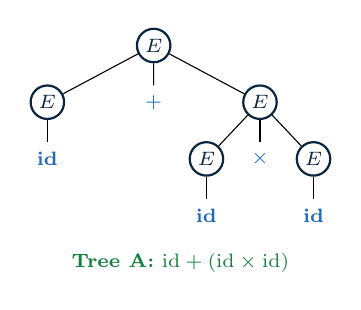
\begin{tikzpicture}[level distance=0.72cm,
          level 1/.style={sibling distance=1.35cm},
          level 2/.style={sibling distance=0.68cm}]
          % Tree 1: Left associative (+) at root
          \node[treeNode] {$E$}
            child {node[treeNode] {$E$} child {node[treeLeaf] {$\text{id}$}}}
            child {node[treeLeaf] {$+$}}
            child {node[treeNode] {$E$}
              child {node[treeNode] {$E$} child {node[treeLeaf] {$\text{id}$}}}
              child {node[treeLeaf] {$\times$}}
              child {node[treeNode] {$E$} child {node[treeLeaf] {$\text{id}$}}}
            };
          \node[below=0.15cm] at (current bounding box.south) {\scriptsize\color{accentGreen}\textbf{Tree A:} $\text{id} + (\text{id} \times \text{id})$};
        \end{tikzpicture}
        \hspace{0.25cm}
        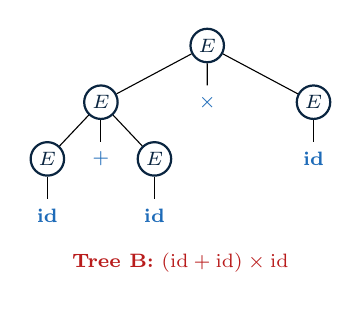
\begin{tikzpicture}[level distance=0.72cm,
          level 1/.style={sibling distance=1.35cm},
          level 2/.style={sibling distance=0.68cm}]
          % Tree 2: Multiplication at root
          \node[treeNode] {$E$}
            child {node[treeNode] {$E$}
              child {node[treeNode] {$E$} child {node[treeLeaf] {$\text{id}$}}}
              child {node[treeLeaf] {$+$}}
              child {node[treeNode] {$E$} child {node[treeLeaf] {$\text{id}$}}}
            }
            child {node[treeLeaf] {$\times$}}
            child {node[treeNode] {$E$} child {node[treeLeaf] {$\text{id}$}}};
          \node[below=0.15cm] at (current bounding box.south) {\scriptsize\color{accentCrimson}\textbf{Tree B:} $(\text{id} + \text{id}) \times \text{id}$};
        \end{tikzpicture}
        }
      \end{center}
      \vspace{-0.15cm}
      \begin{center}
        {\tiny\color{charcoalText}\textbf{Resolution:} Enforce precedence tiers ($E \to E + T \mid T$, $T \to T \times F \mid F$).}
      \end{center}
    \end{column}
  \end{columns}
\end{frame}

% ------------------------------------------------------------------------------
% Slide 5: Week 6: Chomsky Normal Form (CNF)
% ------------------------------------------------------------------------------
\begin{frame}{Week 6: Chomsky Normal Form (CNF)}
  \begin{tcolorbox}[conceptcard]
    {\bfseries\footnotesize\color{gimpanavy} Definition \& Canonical Structure (Sipser Def 2.8)}
    \vspace{0.04cm}
    \footnotesize
    A Context-Free Grammar is in \textbf{Chomsky Normal Form (CNF)} if every rule has one of three forms:
    $$A \to BC \quad\text{or}\quad A \to a \quad\text{or}\quad S \to \varepsilon \quad \text{(where $B, C \in V \setminus \{S\}$ and $a \in \Sigma$)}.$$
  \end{tcolorbox}

  \vspace{0.06cm}
  \begin{columns}[T]
    \begin{column}{0.54\textwidth}
      \colheader{The 4-Step Conversion Algorithm}
      \begin{tcolorbox}[examplecard, top=2.5pt, bottom=2.5pt]
        \begin{enumerate}\setlength{\itemsep}{2pt}\scriptsize
          \item \textbf{New Start Symbol:} Add rule $S_0 \to S$ to prevent the start symbol from appearing on any RHS.
          \item \textbf{Eliminate $\varepsilon$-Rules:} For rule $A \to \varepsilon$, remove it and replace every $R \to uAv$ with $R \to uv$.
          \item \textbf{Eliminate Unit Rules:} For rule $A \to B$, remove it and copy all productions $B \to u$ into $A \to u$.
          \item \textbf{Binarize Long RHS:} Replace $A \to u_1 u_2 \dots u_k$ ($k \ge 3$) with cascade $A \to u_1 C_1, C_1 \to u_2 C_2, \dots$
        \end{enumerate}
      \end{tcolorbox}
    \end{column}

    \hfill

    \begin{column}{0.44\textwidth}
      \colheader{Why CNF Matters for Algorithms}
      \begin{tcolorbox}[spotlightcard, top=3pt, bottom=3pt]
        \begin{itemize}\setlength{\itemsep}{2.5pt}\footnotesize
          \item \textbf{Binary Derivation Bound:} Any string $w \in L(G)$ of length $n = |w| \ge 1$ requires \textbf{exactly $2n - 1$ steps} to derive!
          \item \textbf{Decidability:} Instantly proves CFL membership is decidable (finite search space).
          \item \textbf{CYK Algorithm:} Enables dynamic programming parsing in $\mathcal{O}(n^3)$ polynomial time.
        \end{itemize}
      \end{tcolorbox}
    \end{column}
  \end{columns}
\end{frame}

% ------------------------------------------------------------------------------
% Slide 6: Week 6 Spotlight: Grammar-Guided LLM Decoding (NeurIPS 2023)
% ------------------------------------------------------------------------------
\begin{frame}{Week 6 Spotlight: Grammar-Guided LLM Structured Decoding}
  \begin{tcolorbox}[spotlightcard, top=2pt, bottom=2pt, before=\vspace{0pt}, after=\vspace{2pt}]
    \footnotesize
    \textbf{Seminal Literature (NeurIPS Foundation Models 2023):} 
    \textbf{Willard \& Louf}, \textit{``Efficient Guided Generation for Large Language Models,''} \textbf{NeurIPS 2023} (HuggingFace \texttt{outlines}).
  \end{tcolorbox}

  \vspace{0.04cm}
  \begin{columns}[T]
    \begin{column}{0.48\textwidth}
      \colheader{The Industrial Production Problem}
      \begin{tcolorbox}[alertcard, top=3pt, bottom=3pt]
        \begin{itemize}\setlength{\itemsep}{2.5pt}\footnotesize
          \item \textbf{Malformed JSON / SQL:} Modern LLMs produce syntax errors (missing closing braces, hallucinated keys) in 5--15\% of API calls.
          \item \textbf{Brittle Retries:} Re-prompting adds latency ($\ge 800\text{ms}$) and enterprise billing cost without safety guarantees.
        \end{itemize}
      \end{tcolorbox}
    \end{column}

    \hfill

    \begin{column}{0.48\textwidth}
      \colheader{The Automata Solution: PDA Logit Masking}
      \begin{tcolorbox}[examplecard, top=3pt, bottom=3pt]
        \begin{itemize}\setlength{\itemsep}{2.5pt}\footnotesize
          \item \textbf{Pushdown Grammar Parser:} Compile JSON Schema into an equivalent Pushdown Automaton / CFG parser.
          \item \textbf{Logit Masking:} Mask invalid tokens at decoding step $t$:
            $$\text{Logit}_v = -\infty \quad \forall v \notin \text{NextTokens}(S_t)$$
          \item \textbf{Guarantee:} \textbf{100\% mathematically valid syntax} with zero inference retries!
        \end{itemize}
      \end{tcolorbox}
    \end{column}
  \end{columns}
\end{frame}

% ------------------------------------------------------------------------------
% Slide 7: Week 7: Pushdown Automata (PDAs)
% ------------------------------------------------------------------------------
\begin{frame}{Week 7: Pushdown Automata (PDAs)}
  \begin{columns}[T, onlytextwidth]
    \begin{column}{0.54\textwidth}
      \colheader{Formal 6-Tuple Definition (Sipser Def 2.13)}
      \begin{tcolorbox}[conceptcard]
        \footnotesize
        A \textbf{Nondeterministic Pushdown Automaton (PDA)} is a 6-tuple $\bigl(Q, \Sigma, \Gamma, \delta, q_0, F\bigr)$:
        \begin{enumerate}\setlength{\itemsep}{1.5pt}
          \item $Q$: Finite set of internal \textbf{states}.
          \item $\Sigma$: Finite input \textbf{alphabet}.
          \item $\Gamma$: Finite \textbf{stack alphabet} (storage symbols).
          \item $\delta: Q \times \Sigma_{\varepsilon} \times \Gamma_{\varepsilon} \to \mathcal{P}(Q \times \Gamma_{\varepsilon})$: Transition function.
          \item $q_0 \in Q$: Designated \textbf{start state}.
          \item $F \subseteq Q$: Set of \textbf{accept states}.
        \end{enumerate}
      \end{tcolorbox}
    \end{column}

    \hfill

    \begin{column}{0.44\textwidth}
      \colheader{The LIFO Stack Memory Architecture}
      \vspace{0.05cm}
      \begin{center}
        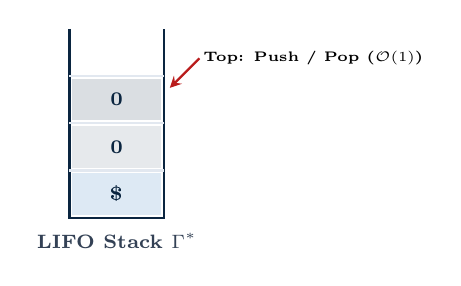
\begin{tikzpicture}[scale=0.75]
          % Stack container
          \draw[thick, draw=gimpanavy] (0, 3.2) -- (0, 0) -- (1.6, 0) -- (1.6, 3.2);
          % Stack elements
          \fill[gimpaaccent!15] (0.05, 0.05) rectangle (1.55, 0.75);
          \node at (0.8, 0.4) {\scriptsize\bfseries\color{gimpanavy}\$};
          \draw[ruleGray, thick] (0, 0.8) -- (1.6, 0.8);
          
          \fill[gimpanavy!10] (0.05, 0.85) rectangle (1.55, 1.55);
          \node at (0.8, 1.2) {\scriptsize\bfseries\color{gimpanavy}0};
          \draw[ruleGray, thick] (0, 1.6) -- (1.6, 1.6);
          
          \fill[gimpanavy!15] (0.05, 1.65) rectangle (1.55, 2.35);
          \node at (0.8, 2.0) {\scriptsize\bfseries\color{gimpanavy}0};
          \draw[ruleGray, thick] (0, 2.4) -- (1.6, 2.4);
          
          % Annotations
          \draw[->, >=stealth, thick, draw=accentCrimson] (2.2, 2.7) -- (1.7, 2.2);
          \node[right] at (2.1, 2.7) {\tiny\textbf{Top: Push / Pop ($\mathcal{O}(1)$)}};
          
          \node[below] at (0.8, -0.1) {\scriptsize\bfseries\color{gimpaslate}LIFO Stack $\Gamma^*$};
        \end{tikzpicture}
      \end{center}
      \vspace{-0.20cm}
      \begin{tcolorbox}[alertcard, top=2pt, bottom=2pt]
        \scriptsize
        \textbf{Stack Limitation:} Infinite capacity, but strictly restricted access. Deep elements cannot be read without popping top symbols!
      \end{tcolorbox}
    \end{column}
  \end{columns}
\end{frame}

% ------------------------------------------------------------------------------
% Slide 8: Week 7: PDA State Diagram & Execution Trace
% ------------------------------------------------------------------------------
\begin{frame}{Week 7: PDA State Diagram: Recognizer for $L = \{0^n 1^n \mid n \ge 0\}$}
  \colheader{Transition Convention: $a, b \to c$ denotes: ``Read input $a$, Pop $b$ from stack, Push $c$ onto stack''}
  \vspace{0.08cm}
  \begin{center}
    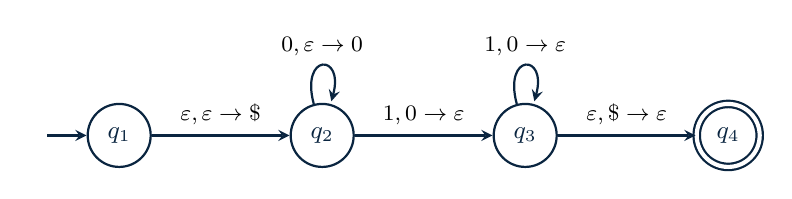
\begin{tikzpicture}[node distance=1.75cm, auto]
      \node[state, initial] (q1) {$q_1$};
      \node[state] (q2) [right=of q1] {$q_2$};
      \node[state] (q3) [right=of q2] {$q_3$};
      \node[state, accepting] (q4) [right=of q3] {$q_4$};

      \path[->]
      (q1) edge node {$\varepsilon, \varepsilon \to \$$} (q2)
      (q2) edge [loop above] node {$0, \varepsilon \to 0$} ()
           edge node {$1, 0 \to \varepsilon$} (q3)
      (q3) edge [loop above] node {$1, 0 \to \varepsilon$} ()
           edge node {$\varepsilon, \$ \to \varepsilon$} (q4);
    \end{tikzpicture}
  \end{center}

  \vspace{-0.15cm}
  \begin{tcolorbox}[examplecard]
    {\bfseries\footnotesize\color{accentGreen} Execution Trace on String $w = 0011$}\par
    \vspace{0.02cm}
    \centering\scriptsize
    \begin{tabular*}{\linewidth}{@{\extracolsep{\fill}} ccccc @{}}
      \toprule
      \textbf{Step} & \textbf{State} & \textbf{Input} & \textbf{Stack} & \textbf{Operation Description} \\
      \midrule
      0 & $q_1$ & $0011$ & $\varepsilon$ & Initial configuration \\
      1 & $q_2$ & $0011$ & $\$$ & Push bottom marker $\$$ \\
      2 & $q_2$ & $011$ & $0\$$ & Read `0', push `0' \\
      3 & $q_2$ & $11$ & $00\$$ & Read `0', push `0' \\
      4 & $q_3$ & $1$ & $0\$$ & Read `1', pop matched `0' \\
      5 & $q_3$ & $\varepsilon$ & $\$$ & Read `1', pop matched `0' \\
      6 & $q_4$ & $\varepsilon$ & $\varepsilon$ & Stack empty; accept state $\implies$ \textbf{ACCEPTED!} \\
      \bottomrule
    \end{tabular*}
  \end{tcolorbox}
\end{frame}

% ------------------------------------------------------------------------------
% Slide 9: Week 7: Fundamental Equivalence: CFG <=> PDA
% ------------------------------------------------------------------------------
\begin{frame}{Week 7: Fundamental Equivalence: $\mathcal{L}(\text{CFG}) = \mathcal{L}(\text{PDA})$}
  \begin{tcolorbox}[conceptcard]
    {\bfseries\footnotesize\color{gimpanavy} Fundamental Theorem of Context-Free Languages (Sipser Thm 2.20)}
    \vspace{0.04cm}
    \footnotesize
    A language $L$ is context-free if and only if some pushdown automaton recognizes it:
    $$\mathcal{L}(\text{CFG}) \equiv \mathcal{L}(\text{PDA}) = \text{Context-Free Languages}.$$
  \end{tcolorbox}

  \vspace{0.06cm}
  \begin{columns}[T]
    \begin{column}{0.48\textwidth}
      \colheader{Direction 1: CFG $\implies$ PDA (Sipser Lemma 2.21)}
      \begin{tcolorbox}[examplecard, top=3pt, bottom=3pt]
        \begin{itemize}\setlength{\itemsep}{2.5pt}\scriptsize
          \item \textbf{Top-Down Simulation:} The PDA simulates the leftmost derivation on its stack.
          \item If top of stack is variable $A$, nondeterministically replace it with RHS of rule $A \to u$.
          \item If top of stack is terminal $a$, match against incoming input symbol and pop.
        \end{itemize}
      \end{tcolorbox}
    \end{column}

    \hfill

    \begin{column}{0.48\textwidth}
      \colheader{Direction 2: PDA $\implies$ CFG (Sipser Lemma 2.27)}
      \begin{tcolorbox}[conceptcard, top=3pt, bottom=3pt]
        \begin{itemize}\setlength{\itemsep}{2.5pt}\scriptsize
          \item \textbf{State Pair Variables:} For every pair of states $(p, q)$, create variable $A_{pq}$ generating all strings driving PDA from $p$ to $q$ with net empty stack.
          \item Compose grammar rules capturing push-pop cycles: $A_{pq} \to a A_{rs} b$ and $A_{pq} \to A_{pr} A_{rq}$.
        \end{itemize}
      \end{tcolorbox}
    \end{column}
  \end{columns}
  
  \vspace{0.08cm}
  \begin{center}
    {\footnotesize\color{charcoalText}\textbf{Compiler Runtime Mirror:} Modern programming call stacks directly implement PDA push-pop semantics.}
  \end{center}
\end{frame}

% ------------------------------------------------------------------------------
% Slide 10: Week 7 Spotlight: Production Parser Generators (PLDI 2011)
% ------------------------------------------------------------------------------
\begin{frame}{Week 7 Spotlight: Production Parser Generators (ANTLR v4)}
  \begin{tcolorbox}[spotlightcard, top=2pt, bottom=2pt, before=\vspace{0pt}, after=\vspace{2pt}]
    \footnotesize
    \textbf{Seminal Literature (ACM SIGPLAN PLDI 2011):} 
    \textbf{Parr et al. (Univ. of San Francisco)}, \textit{``Adaptive $\text{LL}(*)$ Parsing: The Power of Dynamic Analysis,''} \textbf{PLDI 2011}.
  \end{tcolorbox}

  \vspace{0.04cm}
  \begin{columns}[T]
    \begin{column}{0.48\textwidth}
      \colheader{Traditional Theory Limit: Static $\text{LL}(k)$ / $\text{LR}(k)$}
      \begin{tcolorbox}[conceptcard, top=3pt, bottom=3pt]
        \begin{itemize}\setlength{\itemsep}{2.5pt}\footnotesize
          \item \textbf{Fixed Lookahead:} Classical parsers enforce $k = 1$ token lookahead to guarantee deterministic $\mathcal{O}(n)$ parsing.
          \item \textbf{Grammar Refactoring Pain:} Forces software engineers to manually left-factor and eliminate left recursion from their grammars.
        \end{itemize}
      \end{tcolorbox}
    \end{column}

    \hfill

    \begin{column}{0.48\textwidth}
      \colheader{The Systems Solution: Adaptive $\text{LL}(*)$}
      \begin{tcolorbox}[examplecard, top=3pt, bottom=3pt]
        \begin{itemize}\setlength{\itemsep}{2.5pt}\footnotesize
          \item \textbf{Dynamic DFA Lookahead:} ANTLR launches a sub-DFA at runtime to read arbitrary token lookahead only when ambiguity is detected!
          \item \textbf{Industrial Scale:} Powers \textbf{SQLite}, \textbf{PostgreSQL} query engines, \textbf{Java / Python} compilers, and IDE syntax highlighters.
        \end{itemize}
      \end{tcolorbox}
    \end{column}
  \end{columns}
\end{frame}

% ------------------------------------------------------------------------------
% Slide 11: Week 8: The Pumping Lemma for Context-Free Languages
% ------------------------------------------------------------------------------
\begin{frame}{Week 8: The Pumping Lemma for Context-Free Languages}
  \begin{tcolorbox}[conceptcard]
    {\bfseries\footnotesize\color{gimpanavy} Formal Theorem Statement (Sipser Thm 2.34)}
    \vspace{0.04cm}
    \footnotesize
    If $L$ is a Context-Free Language, then there exists a pumping length $p \ge 1$ such that every string $s \in L$ with $|s| \ge p$ can be divided into $s = uvxyz$ satisfying three conditions:
    \begin{enumerate}\setlength{\itemsep}{1pt}
      \item $u v^i x y^i z \in L$ for each $i \ge 0$ \quad (\textbf{Simultaneous Double Pumping Property}),
      \item $|vy| > 0$ \quad (\textbf{At least one of $v$ or $y$ is non-empty}),
      \item $|vxy| \le p$ \quad (\textbf{Pumping Window Bounded by $p$}).
    \end{enumerate}
  \end{tcolorbox}

  \vspace{0.06cm}
  \begin{columns}[T, onlytextwidth]
    \begin{column}{0.48\textwidth}
      \colheader{Parse Tree Geometric Pigeonhole Principle}
      \begin{tcolorbox}[examplecard, top=3pt, bottom=3pt]
        \begin{itemize}\setlength{\itemsep}{2pt}\scriptsize
          \item In a CNF grammar, a parse tree of height $h$ yields $|s| \le 2^{h-1}$.
          \item If $|s| \ge p = 2^{|V| + 1}$, the tree height must exceed $|V| + 1$.
          \item Along the longest path, \textbf{at least one variable $R \in V$ must repeat} by the Pigeonhole Principle!
        \end{itemize}
      \end{tcolorbox}
    \end{column}

    \hfill

    \begin{column}{0.48\textwidth}
      \colheader{Subtree Replacement Mechanics}
      \begin{tcolorbox}[spotlightcard, top=3pt, bottom=3pt]
        \begin{itemize}\setlength{\itemsep}{2pt}\scriptsize
          \item The upper occurrence of $R$ derives $v R y$.
          \item The lower occurrence of $R$ derives $x$.
          \item We can substitute the lower tree with the upper tree ($i \ge 2$) or delete the loop ($i = 0$), producing valid strings $u v^i x y^i z \in L$.
        \end{itemize}
      \end{tcolorbox}
    \end{column}
  \end{columns}
\end{frame}

% ------------------------------------------------------------------------------
% Slide 12: Week 8: Adversarial Contradiction Template: Non-CFLs
% ------------------------------------------------------------------------------
\begin{frame}{Week 8: Adversarial Proof Template: Non-CFLs}
  \begin{tcolorbox}[alertcard]
    {\bfseries\footnotesize\color{accentCrimson} Adversarial Proof Template: Showing $L = \{a^n b^n c^n \mid n \ge 0\}$ is Non-Context-Free}
    \vspace{0.04cm}
    \begin{enumerate}\setlength{\itemsep}{1.5pt}\scriptsize
      \item \textbf{Proof by Contradiction:} Assume $L$ is context-free $\implies$ Pumping Lemma guarantees pumping length $p$.
      \item \textbf{Select String:} Choose $s = a^p b^p c^p \in L$. Note that $|s| = 3p \ge p$.
      \item \textbf{Apply Window Bound ($|vxy| \le p$):} Substring $vxy$ can span at most \textbf{two distinct symbol types} (either $\{a, b\}$ or $\{b, c\}$, never all three $\{a, b, c\}$).
      \item \textbf{Pump Down ($i = 0$):} In string $s' = u v^0 x y^0 z = uxz$, the count of at most two symbols decreases, while the third remains untouched at $p$.
      \item \textbf{Contradiction:} Symbol counts are no longer equal $\implies s' \notin L \implies$ \textbf{$L$ is strictly non-context-free!}
    \end{enumerate}
  \end{tcolorbox}

  \vspace{0.04cm}
  \begin{tcolorbox}[conceptcard, top=2.5pt, bottom=2.5pt]
    \scriptsize
    \textbf{Non-CFL Case 2: Exact Duplication $L = \{ww \mid w \in \{0, 1\}^*\}$.} Requires non-LIFO cross-serial matching; a single stack cannot compare symbols without inverting sequence order.
  \end{tcolorbox}
\end{frame}

% ------------------------------------------------------------------------------
% Slide 13: Week 8 Spotlight: Attention Limits on Dyck Languages (TACL 2020)
% ------------------------------------------------------------------------------
\begin{frame}{Week 8 Spotlight: Self-Attention Limits on Dyck Languages}
  \begin{tcolorbox}[spotlightcard, top=2pt, bottom=2pt, before=\vspace{0pt}, after=\vspace{2pt}]
    \footnotesize
    \textbf{Seminal Literature (Transactions of the ACL 2020):} 
    \textbf{Michael Hahn (Stanford University)}, \textit{``Theoretical Limitations of Self-Attention in Neural Sequence Models,''} \textbf{TACL 2020}.
  \end{tcolorbox}

  \vspace{0.04cm}
  \begin{columns}[T]
    \begin{column}{0.48\textwidth}
      \colheader{The Dyck-$k$ Hierarchical Benchmark}
      \begin{tcolorbox}[conceptcard, top=3pt, bottom=3pt]
        \begin{itemize}\setlength{\itemsep}{2.5pt}\footnotesize
          \item \textbf{Nested Brackets:} Dyck-$k$ consists of properly balanced parentheses: \texttt{[ ( \{ \} ) ]}.
          \item \textbf{Trivial for PDAs:} Solvable in $\mathcal{O}(n)$ linear time with a simple stack push/pop counter.
        \end{itemize}
      \end{tcolorbox}
    \end{column}

    \hfill

    \begin{column}{0.48\textwidth}
      \colheader{Why Standard Transformers Fail}
      \begin{tcolorbox}[alertcard, top=3pt, bottom=3pt]
        \begin{itemize}\setlength{\itemsep}{2.5pt}\footnotesize
          \item \textbf{Circuit Depth Bound ($\mathbf{TC}^0$):} Self-attention with fixed depth lacks recursive state tracking.
          \item \textbf{Theoretical Proof:} Hahn proves that self-attention cannot evaluate hierarchical nesting depth beyond its context window without exponential precision!
        \end{itemize}
      \end{tcolorbox}
    \end{column}
  \end{columns}
\end{frame}

% ------------------------------------------------------------------------------
% Slide 14: Module 2 Summary & Looking Ahead to Module 3
% ------------------------------------------------------------------------------
\begin{frame}{Module 2 Summary \& Looking Ahead to Module 3}
  \begin{columns}[T]
    \begin{column}{0.48\textwidth}
      \colheader{Module 2 Key Scientific Takeaways}
      \begin{tcolorbox}[conceptcard, top=3pt, bottom=3pt]
        \begin{itemize}\setlength{\itemsep}{2.5pt}\footnotesize
          \item \textbf{The Power of Stack Memory:} Pushdown Automata and CFGs elevate computation from flat regular tokens to recursive nested trees (ASTs, JSON).
          \item \textbf{The Boundary of Stack Memory:} A single LIFO stack cannot verify multi-way equality ($a^n b^n c^n$) or cross-serial dependencies ($ww$).
        \end{itemize}
      \end{tcolorbox}
    \end{column}

    \hfill

    \begin{column}{0.48\textwidth}
      \colheader{Looking Ahead: Module 3 (Weeks 9--12)}
      \begin{tcolorbox}[spotlightcard, top=3pt, bottom=3pt]
        \begin{itemize}\setlength{\itemsep}{2.5pt}\footnotesize
          \item \textbf{The Tape Upgrade:} What happens if we replace the restricted LIFO stack with an \textbf{infinite, bidirectional read/write tape}?
          \item \textbf{Turing Completeness:} We enter the realm of unrestricted computation: \textbf{Turing Machines}, the \textbf{Church--Turing Thesis}, and the unbreakable boundary of the \textbf{Halting Problem}!
        \end{itemize}
      \end{tcolorbox}
    \end{column}
  \end{columns}

  \vspace{0.15cm}
  \begin{center}
    {\footnotesize\color{gimpanavy}\textbf{Midterm Exam Preparation:} Comprehensive review of Modules 1 \& 2 in Week 8.}
  \end{center}
\end{frame}

\end{document}
